\section{Plant-wide control}


\subsection{Plant-wide control philosophy and survey table} %0.25 page %Marie

Nitroma aimed at developing an effective plant-wide control structure for the entire chemical plant following a general heuristic procedure proposed by \textcite{}. A plant-wide control approach offers many advantages over an individual unit based approach. Firstly, disturbance propagation introduced by multiple recycle loops in the process can be efficiently mitigated. Secondly, the likelihood of conflicts between control loops is reduced, so highly oscillatory behaviour of any control parameter becomes very unlikely. 

The control objectives and consequences associated with poor control were identified for all major process units. Each potential control loop has a controlled variable, a manipulated variable, a sensor and actuator. All possible disturbances affecting the controlled variable were also listed. Finally the survey addressed major maintenance issues and proposed solutions to mitigate them. The plant wide survey can be found in the Supporting Documentation \Cref{sec:PWS}.


\subsection{Key controls}

\subsubsection{Throughput and quality control} %0.75 page %Stephen
Throughput control is an essential part of Nitroma's control strategy as it ensures that the production capacity of the three products can be consistently met. A general framework for choosing a suitable throughput manipulator (TPM) recommends choosing a valve that directly impacts the primary reactor's reaction rate while having minimal impact on the separation system. This could be achieved by changing the heat removal duty from the reactor, the flowrate of reactants, catalysts, or reactor effluent. The stepwise procedure proposed by \textcite{} aided in the selection process of Nitroma's TPM. 
%Additional consideration has to be given to explicit TPMs (i.e. a valve on a process stream) being in the direction "of" or "opposite to" flow. Having a TPM in direction "of" flow such as a valve on the reactor feed provides the most intuitive and traditional form of control, yet having a TPM in direction "opposite of" flow such as a valve on the reactor effluent may offer greater process stability. 

\paragraph{Identify a primary process path}
From the process flow diagram (see xxxx), the primary process path for each product begins with toluene and nitric acid feed sent to R101 and three separators (S101, S102 and S103) before diverging. The path for o-toluidine leads on from S103 to R201 through to S202. The paths for 4-aminobenzaldehyde and 4-aminobenzoic acid are shared from S103 to S303. The latter product is produced from following S303 to R401, then S401 through to R601 and finally S601. The former will be produced from following S303 to S501, then R501 to S504.  

\paragraph{List candidate TPMs}
Potential TPMs have to lie on the common paths of all the products. This makes the feed and streams between R101, S101, S102 and S103 potential options. \textcite{} recommends a TPM that directly controls the reaction rate in the primary reactor. This can be justified if the separation system is well designed and operating efficiently. Around reactor R101, a choice was made to control an explicit flow rather than an implicit flow such as cooling water flowrate. This is because the nitration reaction in R101 is highly exothermic and perturbations to the heat removal by the cooling water increases the risk of thermal runaway and further hazardous consequences. 

\paragraph{Prefer internal flows}
The feed flow rate to R101 was selected as the TPM as it would directly affect the inventory in the reactor. This would make it easier to control the reactor in the unlikely event that the reactor was becoming unstable due to temperature buildup. Pump 101 was used to control the feed flow rate.

To ensure the products from the plant were reliably meeting quality specifications, composition analysers were installed after major reactors and separators in the plant, and inferential sensors such as density or temperature were used to increase reliability of these measurements. Good control of the selectivity in the reactors was achieved by robust control of the pressure and temperature. Ratio controllers maintained correct feed ratios to reactors.

\subsubsection{Inventory and recycle loops control} %0.25page %Stephen
    \begin{wrapfigure}{r}{0.5\linewidth}
        \centering
        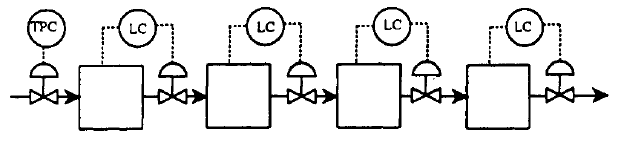
\includegraphics[width=\linewidth]{chapters/4-operation-control/4-Figures/TPM-Price-1994.png}
        \caption{Example of inventory control in direction of flow, taken from \textcite{}}
        \label{fig:TPM}
    \end{wrapfigure}
Inventory control is important to maintain a steady operation of the plant with no accumulation of material in any process unit. Effective inventory controllers are those that are on the primary path, and thus exclude recycle streams. Since the TPM was at the feed to the process, all inventory controls were placed in the direction of flow in order to ensure changes to the production rate from the TPM are propagated throughout the process (see Figure \ref{fig:TPM}). 

Purge streams were added in every recycle loop to prevent the buildup of non-reactive components in process streams.  


\subsection{Challenges to control}%Marie

\subsubsection{Difficult measurements and dynamics} %0.75 page
Composition analysis presents the first difficult measurement. Though an essential technique to ensure product specifications are met, its long measurement process leads to a long time delay between the apparition of a deviation, its identification by the composition transmitter and its resolution via the control loops in place. Where possible inferential control can be implemented to reduce the time delay. For instance, the bottoms composition of the distillation column can be controlled with temperature []. However, effective inferential control requires robust calibration curves between the measured and controlled variable, but these can be generated using experimental data. Moreover, the presence of impurities can significantly impact correlations, but this can be mitigated by relying on measurements from multiple inferential sensors such as density and viscosity measurements in addition to temperature [].

Secondly, the robust control of reactor temperatures is one of Nitroma's major concerns since all reactions are highly exothermic and could lead to thermal runaways. More specifically, in the nitration reactor R101, a hot spot can form at the centre of the catalyst bed in the shell-and-tube heat exchanger reactor, which means it can not be directly measured with temperature transmitters placed at the walls. It is suggested to conduct experiments and modelling work to develop correlations between the reactor wall temperature and the inner temperature. Additionally, the monitoring of cooling water outlet temperature can infer of the presence of a significant increase in temperature in the reactor.

Difficult dynamics can also be encountered while conducting a plant-wide control structure. Since Nitroma's process is continuous, it is expected that less difficult control dynamics will be found as opposed to a batch process. Nonetheless, it is necessary to have dynamic modelling of plant to be able to design better control loops and transfer functions.


\subsubsection{Process bottleneck} % 0.25 page
The nitration reactor R101 is Nitroma's process bottleneck since it produces the precursors for all three end products. As the first major unit in the process, any issue encountered in its operation would cascade through the whole plant. The operational conditions of this reactor determines the proportions of the three products, as well as the final quantity and purity which can be obtained. Hence, safety functions were installed to closely monitor and control operational parameters (temperature, pressure, flow and composition). To further avoid the propagation of quality disturbances to downstream units, buffer tanks are installed before each reactor in the process. In addition to regular maintenance and inspection of the equipment for fouling and early catalyst deactivation, a back-up cooling system is implemented to reduce as much as reasonably feasible the risk of thermal runaway.


\subsection{Key disturbances} % 0.75 page

\subsubsection{Feed quality}
The quality of the toluene, nitric acid, formic acid, hydrogen air and methanol used in the process can significantly affect the good operation of the system. In addition to lowering the final product quality, impurities present in the feeds can decrease catalyst activity in the reactors, thus resulting in lower production and off-specification products. Mitigating strategies include the installation of feed composition analysers and a procedure to ensure storage tanks are correctly sealed. It is also recommended to use air scrubbers to purify the air used for the oxidation of PNT.

\subsubsection{Flowrate}
Variations in flowrates are one of the most prevalent disturbances in the process. Not only can they affect the overall throughput and quality, uncontrolled changes in flowrate can also pose serious safety issues. A significant drop in cooling water flowrate could result in a thermal runaway if the exothermic reactions cannot be managed adequately. The feedforward control loops installed in the plant aim at helping the system to proactively adjust to upstream flowrate disturbances. The installation of back-up auxiliary equipment, such as back-up pumps, also contributes to the plant's ability to withstand flowrate disturbances.

\subsubsection{Ambient temperature}
The ambient temperature can affect the plant operation in multiple ways. Firstly, it can impact the temperature of the cooling water to the exothermic reactors. Ineffective control of the heat removal duty could lead to thermal runaway. Secondly, air is the oxidiser in the partial and complete oxidation of PNT (reactors R301 and R401) and thus its temperature will directly affect reaction rates. Finally, streams that are cooled in an air heat exchanger, such as the cooler in the Rankine cycle around the PNT crystalliser will see product purity negatively affected if sufficient cooling cannot be achieved. 

To limit the impact of ambient air temperature on the process, ambient temperature transmitters are installed on the plant and connected to feedfoward control loops on major units. Units that depend on tight temperature control (exothermic reactors, crystallisers) have back-up cooling systems using a different cooling medium such as the refrigerant R1234ze. This would require the installation of a back-up Rankine cycle for the cooling system. Another contingency is the construction of cooling towers to provide sufficiently cold cooling water when the normal cooling water supplier fails to deliver the requirements.

\subsubsection{Utilities}
The main disturbances in key utilities include the supply of electricity and the temperature and flowrate of cooling water and steam. The fluctuations in the latter have already been discussed in the previous section and can be mitigated via feedforward control.

Electricity supplies heat to process fluids through electric heaters, runs the pumps and fans and also the automated control loops. If power is lost, back-up battery packs provide the energy required to bring the equipment and control valves to a fail-safe state, thus preventing accidents. Restarting the plant upon electrical power restoration must be correctly managed to prevent the automatic restart of some equipment before other sections are ready for operation. The installation of a robust interlock system accompanied with back-up power supplies can accommodate with temporary losses of power. However in prevision of longer outages, procedures to bring the plant to a safe state must be implemented.


\subsection{Key areas of maintenance} %0.25 page
One regular maintenance step is to remedy catalyst deactivation. The four reactions involved in Nitroma's process indeed use solid catalysts whose catalytic activity can be weakened by time and impurities. Catalysts can be regenerated during planed shutdown to ensure optimum process performance. Another major operation taking place during maintenance is the inspection of electrical appliances, in particular control instruments and electric heaters. The transmitters and their associated control loops and alarms will need to be calibrated and tested. In addition, the heating elements are inspected to assess their level of wear and tear. Finally, fouling can cause major issues in mechanical integrity of the equipment. Fouling is particularly relevant for the crystallisers as solids could accumulate on the walls, reducing heat transfer and the performance. Fouling prevention involves regular inspection of the equipment using ultrasound checks and regular cleaning.